
\documentclass[12pt]{article}

% -- Packages
\usepackage{lscape} 

\usepackage{amsmath}
\usepackage{amsthm}
\usepackage{amssymb}
\usepackage{graphicx}
\usepackage{float}
\usepackage{multirow}
\usepackage{xcolor}
\usepackage{algorithmic}
\usepackage[ruled,vlined,commentsnumbered,titlenotnumbered]{algorithm2e}
\usepackage{array}
\usepackage{booktabs}
\usepackage{url}
\usepackage{parskip}
\usepackage[margin=1in]{geometry}
\usepackage[T1]{fontenc}
\usepackage{cmbright}
\usepackage[many]{tcolorbox}
\usepackage{enumitem}
\usepackage{hyperref}
\usepackage[font=small,labelfont=bf]{caption}
\documentclass{article}
\usepackage[table,xcdraw]{xcolor}
% -- Macros

\newcommand{\HWNum}{5}
\newcommand{\Rule}{\rule{\linewidth}{0.5pt}}
\newcommand{\Expecting}[1]{[\textbf{We are expecting:} #1]}
\newcommand{\Points}[1]{\textbf{(#1 pt.)}}


\begin{document}
\section{\bf User Interface}
\begin{table}[H]
\begin{tabular} {|m{6em}|m{12cm}|}
\hline
Interface ID & I01 \\ \hline
\newline
Name & Add Employee \\ \hline

UI Screen &\newline 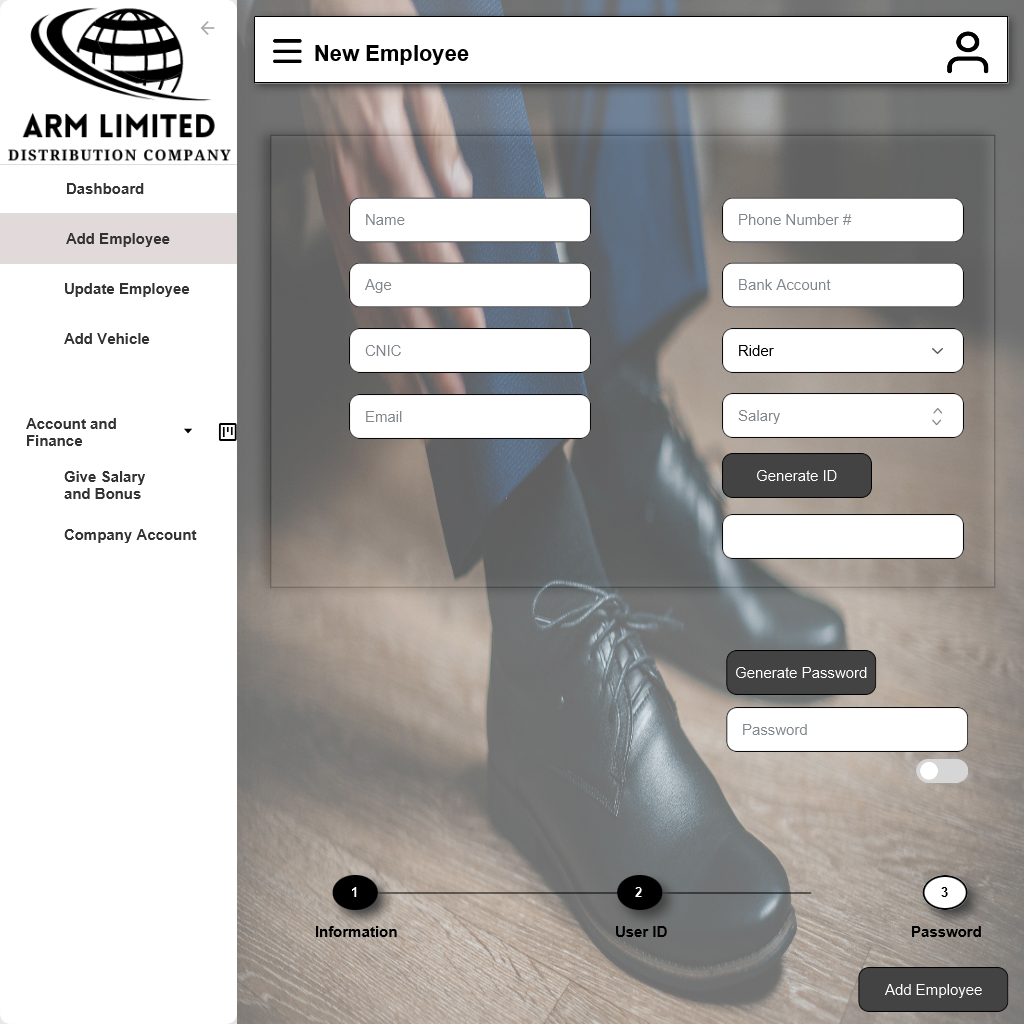
\includegraphics [width=10cm, height=5cm] {first.png} \\ \hline

Validators & 1.	Name: Name should be entered in string.
\newline
2.	Phone Number: It would be of string type with minimum 11 words.
\newline
3.	Age: It would be of int type ranges from 0 to 120.
\newline
4.	Bank Account: It should be input of integers with atleast 15 numbers.
\newline
5.	CNIC: CNIC will be of string type with 13 characters.
\newline
6.	Category: Manager can either select Rider, Supervisor, Sales agent.
\newline
7.	Email: Email will be validated with @gmail.com and it is of string type.
\newline
8.	Salary: It is of int type.
\newline
9.	ID: It is of string type.
\newline
10.	Password: It is of string type.
\newline
. \\ \hline 
\end{tabular}

\end{table}
%%%%%%%%%%%%%%%%%%%%%%%%%%%%%%%%%%%%%%%%%%%%%%%%%%%%%%%%%%%%%%%%%
\begin{table}[H] 
\begin{tabular} {|m{6em}|m{12cm}|}
\hline
Interface ID & I02 \\ \hline
\newline
Name & Update Employee \\ \hline
LinkedUseCase & U06 \\ \hline
UI Screen &\newline 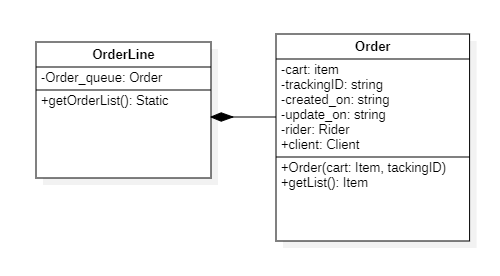
\includegraphics [width=10cm, height=5cm] {2.png} \\ \hline
\end{tabular}
\end{table}
%%continue table on next page
\begin{table}[H] 
\begin{tabular} {|m{6em}|m{12cm}|}
\hline
     & \newline\newline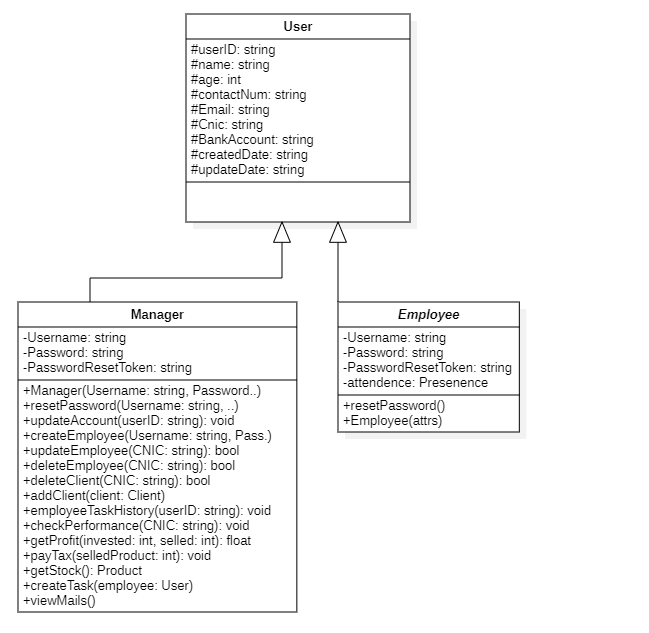
\includegraphics [width=10cm, height=5cm] {3.png}
     \\ \hline
\newline
Validators &  1.Name: Name should be entered in string.
\newline
2.Phone Number: It would be of string type with minimum 11 words.
\newline
3.Age: It would be of int type ranges from 0 to 120.
\newline
4.Bank Account: It should be input of integers with atleast 15 numbers.
\newline
5.CNIC: CNIC will be of string type with 13 characters.
\newline
6.Category: Manager can either select Rider, Supervisor, Sales agent.
\newline
7.Email: Email will be validated with @gmail.com and it is of string type.
\newline
8.Salary: It is of int type.
\newline
9.ID: It is of string type.
\newline
10.Password: It is of string type.
\newline
\\ \hline
\end{tabular}
\end{table}
%%%%%%%%%%%%%%%%%%%%%%%%%%%%%%%%%%%%%%%%%%%%%%%%%%%%%%%%%
\begin{table}[H] 
\begin{tabular} {|m{6em}|m{12cm}|}
\hline
Interface ID & I03 \\ \hline
\newline
Name & Give Salary and Bonus\\ \hline
LinkedUseCase & U04, U05 \\ \hline
UI Screen &\newline 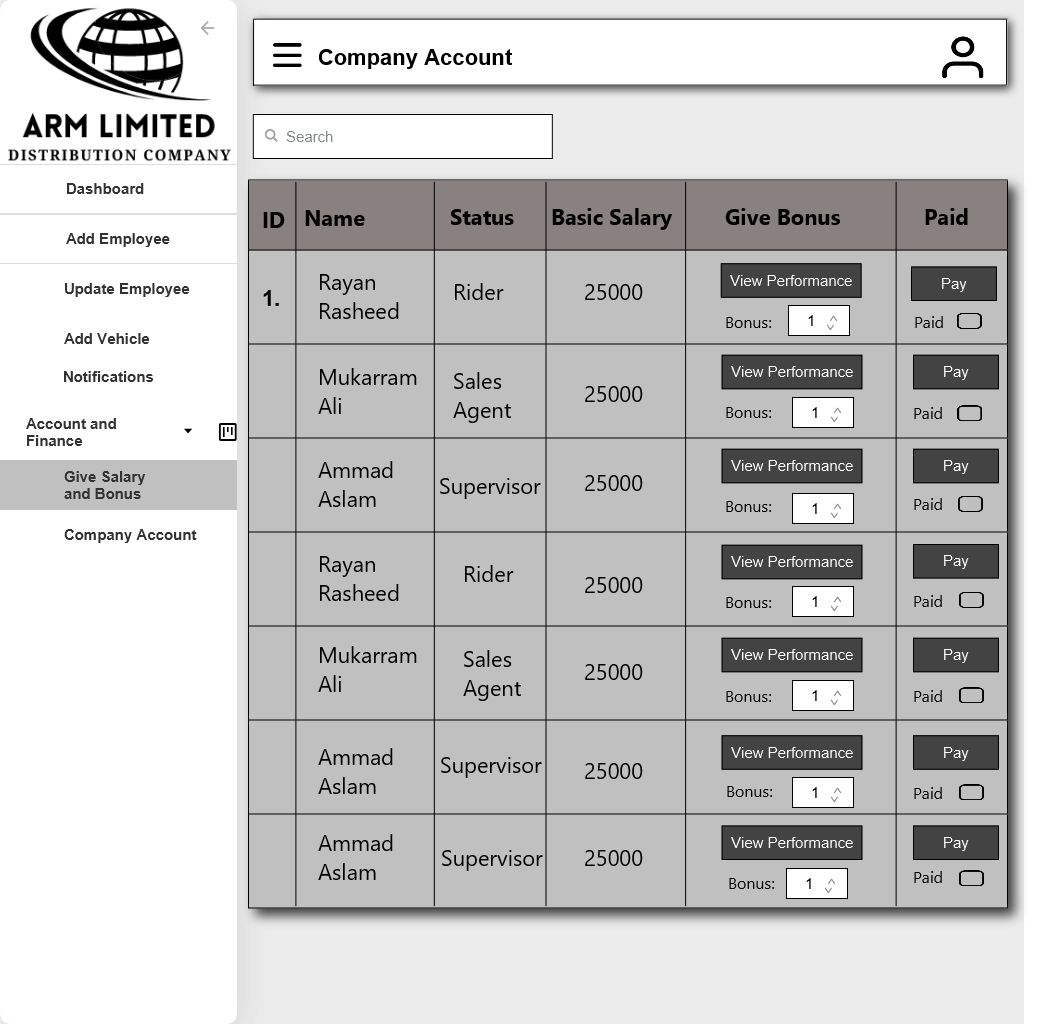
\includegraphics [width=10cm, height=5cm] {r.png} \\ \hline
Validators &  1. Searching: Searching will be according to the name of the employee.
\newline
2. Checkbox: If the salary is paid then it will be checked otherwise it will be unchecked.
\newline
3. Bonus: It should be of int type.
\\ \hline
\end{tabular}
\end{table}
%%%%%%%%%%%%%%%%%%%%%%%%%%%%%%%%%%%%%%%%%%%%%%%%%%%%%%%%%%%%%%%%%5
\begin{table}[H] 
\begin{tabular} {|m{6em}|m{12cm}|}
\hline
Interface ID & I04 \\ \hline
\newline
Name & Company account\\ \hline
LinkedUseCase & U03 \\ \hline
UI Screen &\newline 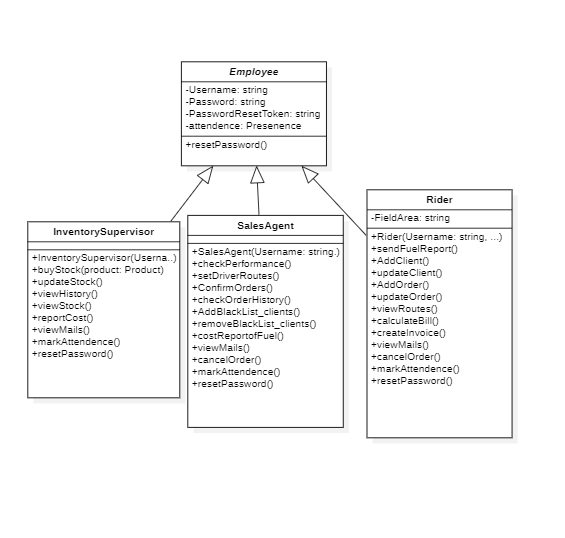
\includegraphics [width=10cm, height=5cm] {4.png} \\ \hline
Validators &  1. Select Category: It is of dropdown menu that contains the value of string type.
\newline
2. Company Total: It contain the company total in int.
\\ \hline
\end{tabular}
\end{table}
%%%%%%%%%%%%%%%%%%%%%%%%%%%%%%%%%%%%%%%%%%%%%%%%%%%%%%%%%%%%%%%%
\begin{table}[H] 
\begin{tabular} {|m{6em}|m{12cm}|}
\hline
Interface ID & I05 \\ \hline
\newline
Name & Buy Stock\\ \hline
LinkedUseCase & U09 \\ \hline
UI Screen &\newline 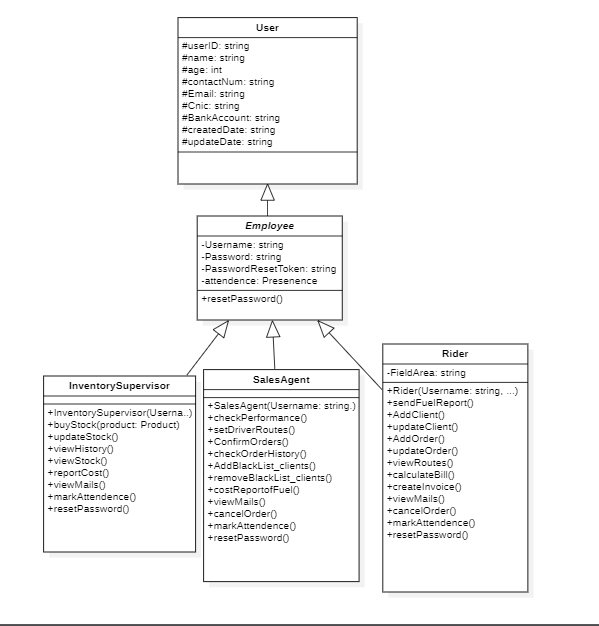
\includegraphics [width=10cm, height=5cm] {5.png} \\ \hline
Validators &  1. Select Quantity: It is int type.
\newline
2. Select Size: It is int type
3. Price: It is of int type
4. Total Amount: It is of int type
\\ \hline
\end{tabular}
\end{table}
%%%%%%%%%%%%%%%%%%%%%%%%%%%%%%%%%%%%%%%%%%%%%%%%%%%%%5

\begin{table}[H] 
\begin{tabular} {|m{6em}|m{12cm}|}
\hline
Interface ID & I06 \\ \hline
\newline
Name & Update Stock\\ \hline
LinkedUseCase & U10 \\ \hline
UI Screen &\newline 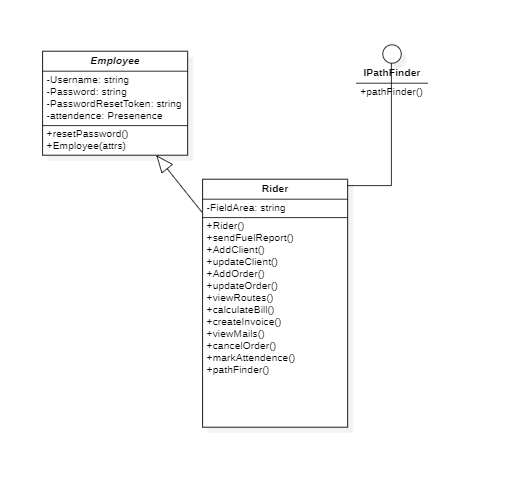
\includegraphics [width=10cm, height=5cm] {6.png} \\ \hline
Validators &  1. Check out button will be working when the order will be delivered.
\\ \hline
\end{tabular}
\end{table}

%%%%%%%%%%%%%%%%%%%%%%%%%%%%%%%%%%%%%%%%%%%%%%%%%%%%%%%%%%%%%%%%%
\begin{table}[H] 
\begin{tabular} {|m{6em}|m{12cm}|}
\hline
Interface ID & I07 \\ \hline
\newline
Name & View History\\ \hline
LinkedUseCase &  U21 \\ \hline
UI Screen &\newline 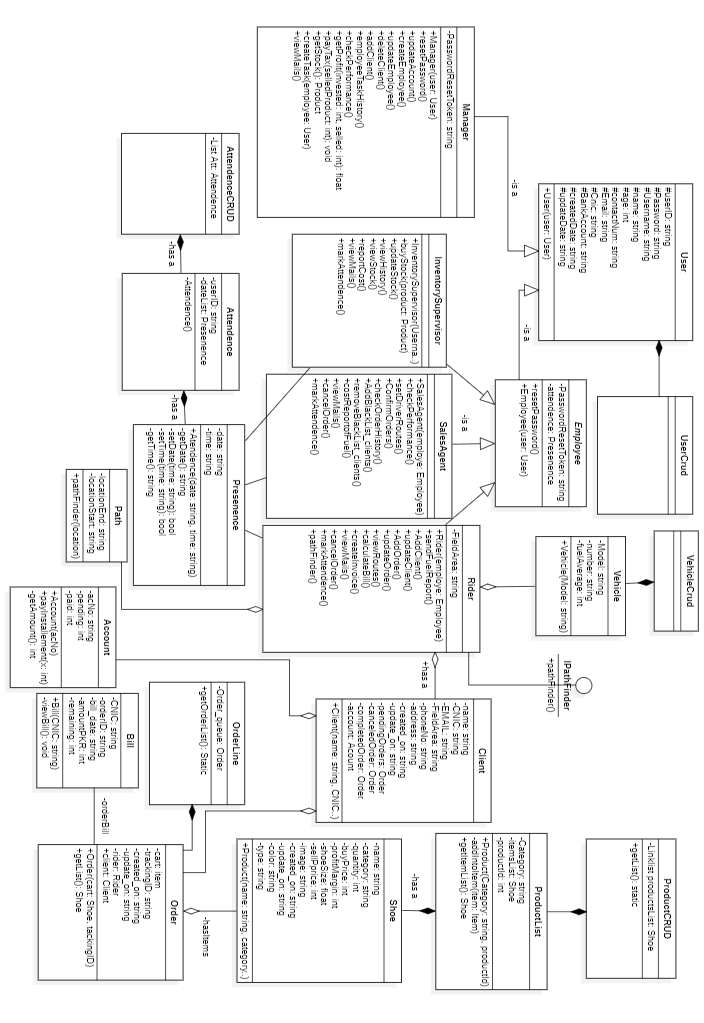
\includegraphics [width=10cm, height=5cm] {8.png} \\ \hline

\end{tabular}
\end{table}
%%%%%%%%%%%%%%%%%%%%%%%%%%%%%%%%%%%%%%%%%%%%%%%%%%%%%%%%%%%%%%%%%%%%%%%%%%%%%
\begin{table}[H] 
\begin{tabular} {|m{6em}|m{12cm}|}
\hline
Interface ID & I08 \\ \hline
\newline
Name & View Stock\\ \hline
LinkedUseCase & U22  \\ \hline
UI Screen &\newline 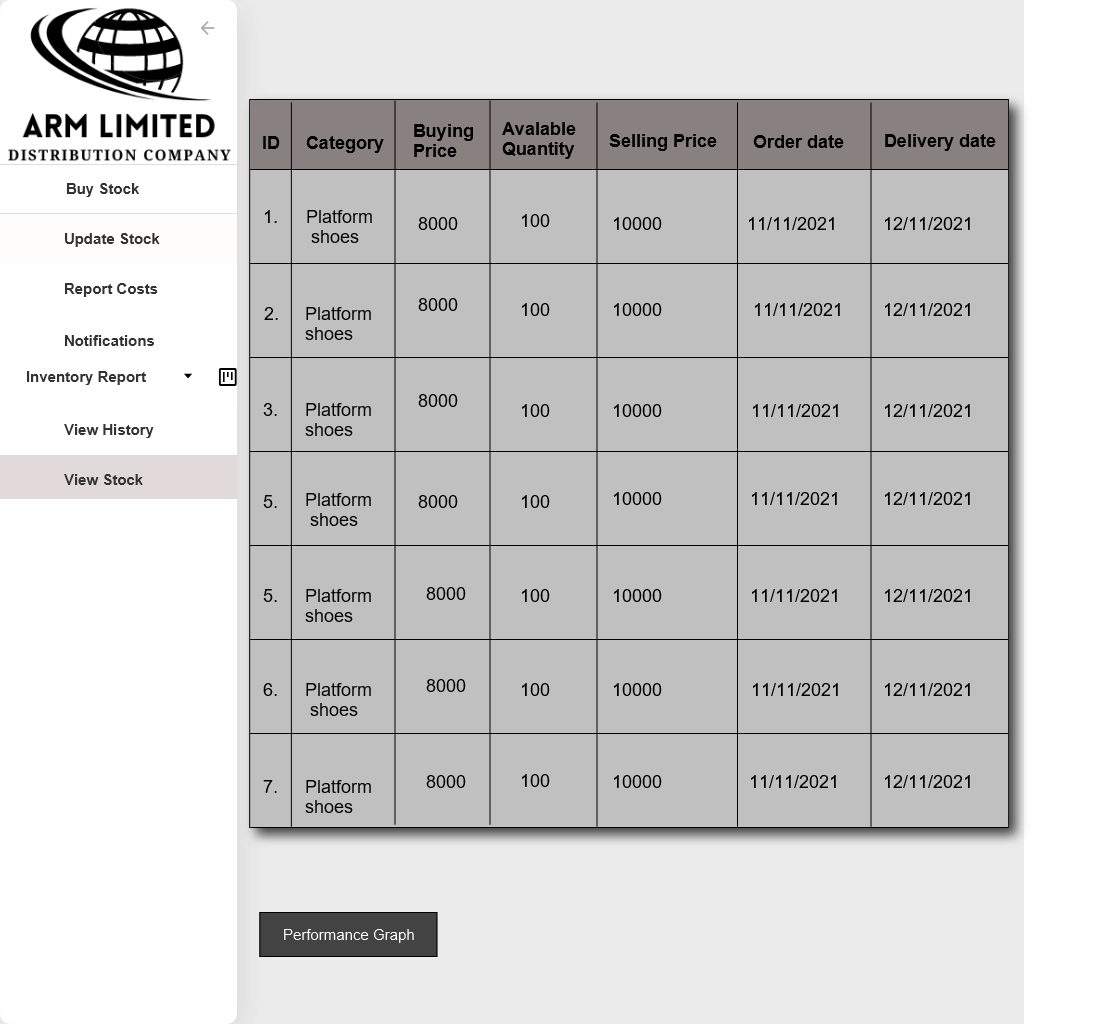
\includegraphics [width=10cm, height=5cm] {9.png} \\ \hline

\end{tabular}
\end{table}
%%%%%%%%%%%%%%%%%%%%%%%%%%%%%%%%%%%%%%%%%%%%%%%%%%%%%%%%%%%%
\begin{table}[H] 
\begin{tabular} {|m{6em}|m{12cm}|}
\hline
Interface ID & I09 \\ \hline
\newline
Name & Report Costs\\ \hline
LinkedUseCase & U12 \\ \hline
UI Screen &\newline 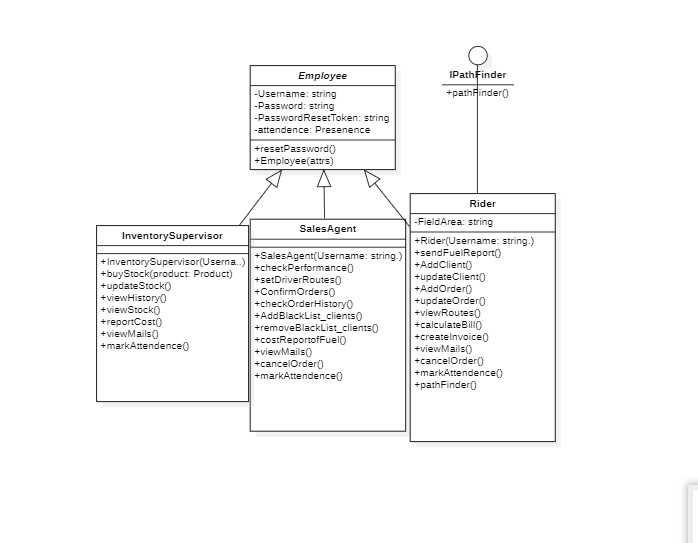
\includegraphics [width=10cm, height=5cm] {7.png} \\ \hline
Validators &  1. Name is of string type.
\newline
2. Price is of int type
\newline
3. Taxes are of float type.
\newline
4. Profit margin is also of float type.
\newline
5. Selling price is also of float type.
\\ \hline
\end{tabular}
\end{table}
%%%%%%%%%%%%%%%%%%%%%%%%%%%%%%%%%%%%%%%%%%%%%%


\end{document}